\documentclass[a4paper,11pt]{ltjsarticle}
\usepackage{graphicx}
\usepackage{luatexja-fontspec}
\usepackage{caption}
\usepackage{amsmath,amssymb,bm,braket}
\usepackage[english]{babel}
\usepackage{multicol}
\usepackage{titlesec}
%\usepackage{gnuplot-lua-tikz}
\usepackage[top=20truemm,bottom=20truemm,left=20truemm,right=20truemm]{geometry}
\usepackage{array}
\usepackage{upgreek}
\usepackage{fancyhdr}
\renewcommand{\refname}{}
\usepackage{listings,jvlisting}
\usepackage{tikz}
\usepackage[thmmarks,amsmath]{ntheorem}
\usepackage[version=3]{mhchem}
\usetikzlibrary{external}
\tikzexternalize
\lstset{
  basicstyle={\ttfamily},
  identifierstyle={\small},
  commentstyle={\smallitshape},
  keywordstyle={\small\bfseries},
  ndkeywordstyle={\small},
  stringstyle={\small\ttfamily},
  frame={tb},
  breaklines=true,
  columns=[l]{fullflexible},
  numbers=left,
  xrightmargin=0pt,
  xleftmargin=3pt,
  numberstyle={\scriptsize},
  stepnumber=1,
  numbersep=1pt,
  lineskip=-0.5ex
}
\captionsetup[figure]{format=plain, labelformat=simple, labelsep=quad,labelfont=bf,name={Fig.}}
\captionsetup[table]{format=plain, labelformat=simple, labelsep=quad,labelfont=bf}
\parindent = 0pt
%[BoldFont=HGSMinchoE]{MSMincho}[BoldFont=HiraMinProN-W6]{HiraMinPro-W3}
\titleformat{\section}{\normalfont\fontsize{9}{10}\bfseries\fontspec{Times New Roman}}{\thesection.}{1em}{}
\usepackage[backend=biber,sorting=none,style=numeric,maxnames=99,minnames=1]{biblatex}
\addbibresource{utility/REFERENCES.bib}
\defbibheading{bibliography}[\refname]{%
  \section*{REFERENCES}%
  \vspace{-7pt}  % ここで空白を調整。お好みの値に変更してください。
}
\newfontfamily\subsectionfont{Times New Roman} % サブセクション用フォント
\titleformat{\subsection}
  {\normalfont\large\bfseries} % サブセクションのフォントを指定
  {\thesubsection}{1em}{}
\renewbibmacro{in:}{}
\renewbibmacro*{journal+issuetitle}{%
  \addcomma\space% カンマとスペースを追加
  \usebibmacro{journal}%
  \setunit*{\addspace}%
  \usebibmacro{volume+number+eid}%
  \setunit{\addspace}%
  \printfield{note}%
  \newunit
}
\renewbibmacro*{volume+number+eid}{
  \printfield{volume}%
  \setunit*{\addnbspace}%
  \printfield{number}%
  \setunit{\addcomma\space}%
  \printfield{eid}
}
\DeclareFieldFormat[article]{volume}{\textbf{#1}}
\DeclareFieldFormat[article]{pages}{#1}
\DeclareFieldFormat{journaltitle}{#1}
\usepackage{hyperref}
\renewenvironment{abstract}{\par\noindent}{\par}
%\pagenumbering{gobble}
\usepackage{docmute}
\usepackage{setspace}
\usepackage{titlesec} % 見出しのカスタマイズ用

% セクションのフォーマットをカスタマイズ
\titleformat{\section}
  {} % フォントサイズとスタイル
  {\Large\bfseries\thesection\ \ }               % 番号の前の内容(空白)
  {0em}            % 番号とタイトルの間の間隔
  {\Large\bfseries}


\theoremstyle{plain}
\theoremheaderfont{\normalfont\bfseries}
\theorembodyfont{\itshape}   % 本文を斜体に
\theoremseparator{.}         % タイトルと本文の区切りを「.」に設定
\newtheorem{definition}{Definition}
\begin{document}
\section{Basics of Quantum Computation}{
    \subsection{Qubits \cite{devitt2013}}\label{qubits}{
        \ \ \ The fundamental unit of quantum information is the qubit. Unlike a classical bit, a qubit can exist in a coherent superposition of its two states, denoted as $\ket{0}$ and $\ket{1}$. These fundamental states are physically realized as charge states in superconducting circuits, the spin of an electron in quantum dots, or atomic spin states. An arbitrary state$\ket{\psi}$ for qubits are expressed as:
        \begin{align}
            \ket{\psi}=\alpha\ket{0}+\beta\ket{1}
        \end{align}
        where $\ket{0}$ and $\ket{1}$ are two orthogonal basis states in hilbert space $\mathcal{H}$ and $|\alpha|^2+|\beta|^2=1$. In the state vector representation, $\ket{0}$ and $\ket{1}$ are commonly expressed as:
        \begin{align}
            \ket{0} =\left(\begin{array}{c}
                1\\
                0
            \end{array}\right),\ \ \ 
            \ket{1} =\left(\begin{array}{c}
                0\\
                1
            \end{array}\right).
        \end{align}
        \ \ \ Unlike classical processing, quantum gates acting on the Hilbert space of qubits must conserve the probability of the qubit states and are therefore unitary. we can define individual qubit gate $I, X, Y$ and $Z$ called pauli gate. These gates have the following properties:
        \begin{align}
            &I\ket{0}=\ket{0},\ \ \ I\ket{1}=\ket{1},\nonumber\\
            &X\ket{0}=\ket{1},\ \ \ X\ket{1}=\ket{0},\\
            &Y\ket{0}=-i\ket{1},\ \ \ Y\ket{1}=i\ket{0},\nonumber\\
            &Z\ket{0}=\ket{0},\ \ \ Z\ket{1}=-\ket{1}\nonumber
        \end{align}
        where $i$ is the imaginary unit. Thus, $I$ is called the identity matrix and acts on a qubit trivially. From Eq. (3), one can derive the matrix representations of the $I$, $X$, $Y$ and $Z$ gates as:
        \begin{align}
            I=\left(\begin{array}{cc}
                1&0\\
                0&1
            \end{array}\right),\ \ \ 
            X=\left(\begin{array}{cc}
                0&1\\
                1&0
            \end{array}\right),\ \ \ 
            Y=\left(\begin{array}{cc}
                0&-i\\
                i&0
            \end{array}\right),\ \ \ 
            Z=\left(\begin{array}{cc}
                1&0\\
                0&-1
            \end{array}\right).
        \end{align}
        \ \ \ If we have multiple qubits, for example, two qubits with states $\ket{0}$ and $\ket{1}$, we represent their combined state using the Kronecker product symbol $\otimes$ as $\ket{0} \otimes \ket{1} = \ket{01}$. In the same way, if we have $n$ states of $\ket{0}$, we represent these states as $\ket{00\cdots 0}$. For short, we denote it as $\ket{0}^n$. Additionally, we can define mutiple qubits gate $G$ as:
        \begin{align}
            G = \bigotimes^n_{i=1}{P_i}=P_1\otimes P_2\otimes\cdots \otimes P_n=P_1P_2\cdots P_n
        \end{align}
        where $P_j$ is single qubit gate for $j$th qubit.
    }
    \subsection{Gates}\label{gates}{
        In Section \ref{qubits}, we introduced only the Pauli gates $I$, $X$, $Y$, and $Z$. The $n$-qubit Pauli gates are denoted as a group $\mathcal{P}_n$. There exist additional gates, which can be classified as either Clifford or non-Clifford gates. The definitions of Clifford gates and non-Clifford gates are given as follows.

        \begin{definition}\label{clifford_group}
            A group of $n$-qubit Clifford gates $\mathcal{C}_n$ is defined as:
            \begin{align}
                \mathcal{C}_n = \{V \in U(n) \mid V \mathcal{P}_n V^\dagger \in \mathcal{P}_n\},
            \end{align}
            where $U(n)$ denotes the $n$-qubit unitary group. Non-Clifford gates belong to a group disjoint from the Clifford group.
        \end{definition}
        In the context of quantum computing, we often use various Clifford and non-Clifford gates to construct circuits. The circuit diagrams and matrix representations of these gates are shown in Fig.~\ref{clifford_and_nonclifford}. An operator is synonymous with a gate in the context of quantum computing. One can verify that $X$, $Y$, $Z$, $H$, $S$, $CNOT$, and $CZ$ are Clifford gates, while $T$ and $CCX$ are non-Clifford gates, as defined in Definition\ref{clifford_group}.

        \begin{table}[h]
            \centering
            \caption{ }
            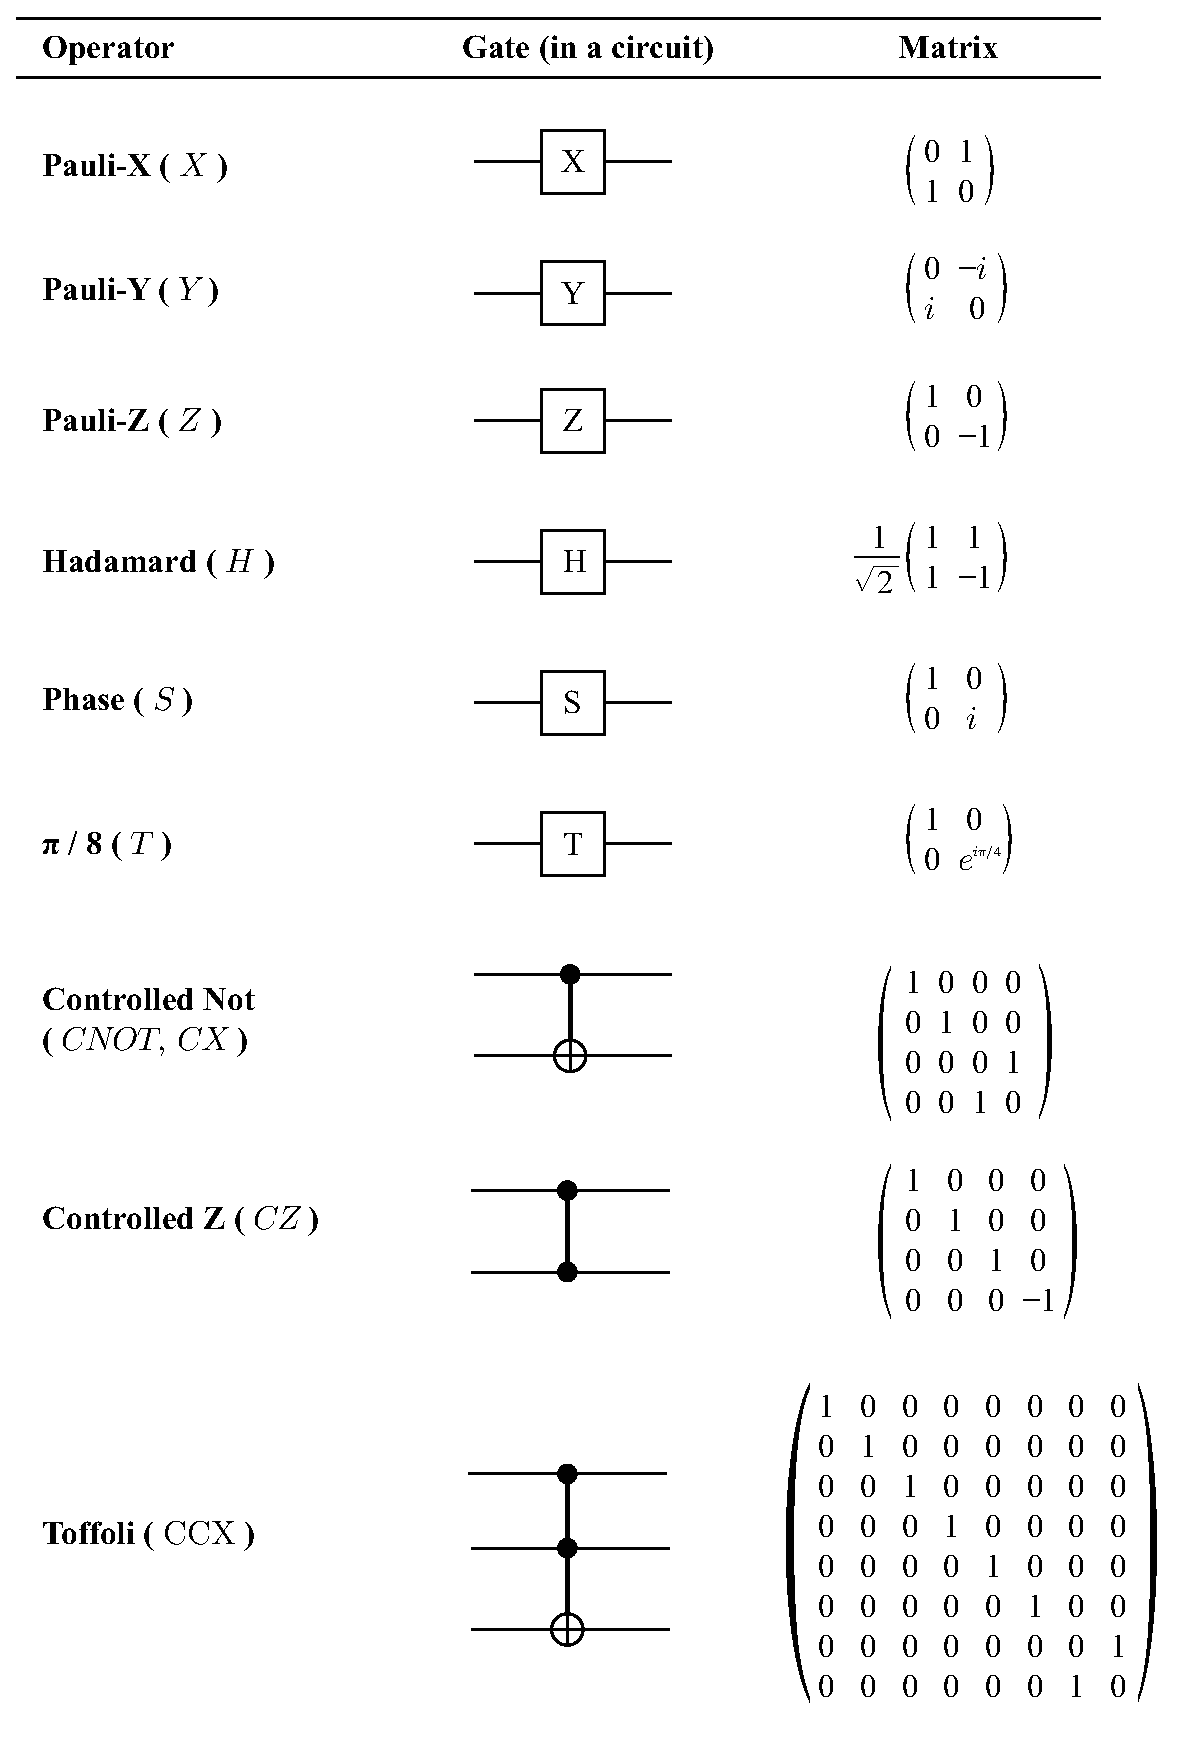
\includegraphics[scale=0.65]{figure/clifford_and_nonclifford.eps}
            \label{clifford_and_nonclifford}
        \end{table}

        \clearpage

        \ \ \ When we use only Clifford gates, we perform only Clifford operations. However, it has been proven that Clifford operations can be efficiently simulated on a classical computer, as stated in the Gottesman-Knill theorem \cite{gottesman1998}. To achieve quantum supremacy, we must use non-Clifford operations for universal computation. However, such non-Clifford operations are very costly because they cannot be error-corrected in quantum error correction theory. To implement non-Clifford operations, we must perform magic state distillation \cite{litinski2019}.
    }
}

\end{document}